\documentclass[conference]{IEEEtran}

\usepackage{ifpdf}
\usepackage{cite}
\ifCLASSINFOpdf
   \usepackage[pdftex]{graphicx}
\else
   \usepackage[dvips]{graphicx}
\fi
\usepackage{amsmath}
\ifCLASSOPTIONcompsoc
  \usepackage[caption=false,font=normalsize,labelfont=sf,textfont=sf]{subfig}
\else
  \usepackage[caption=false,font=footnotesize]{subfig}
\fi
\usepackage{url}
\usepackage{xcolor}

\hyphenation{op-tical net-works semi-conduc-tor}

\pagestyle{empty}

\usepackage{booktabs}
\usepackage{amsmath}
\usepackage{subfig}
\usepackage[ruled,vlined,linesnumbered]{algorithm2e}

\newcommand{\eg}{{\it e.g.}}
\newcommand{\aka}{{\it a.k.a.}}
\newcommand{\etal}{{\it et al.}}
\newcommand{\etc}{{\it etc}}
\newcommand{\ie}{{\it i.e.}}

\begin{document}

\title{DIAL: Distributed Elephant Flow Counting on SDN}

\author{\IEEEauthorblockN{Zheng Peng,
Hao Li and
Chengchen Hu}
\IEEEauthorblockA{Department of Computer Science and Technology\\
Xi'an Jiaotong University\\
Email: pengzheng@stu.xjtu.edu.cn, \{hao.li, chengchenhu\}@xjtu.edu.cn}}

\maketitle

\begin{abstract}
In network measurement, many statistics counters need maintaining on the switch and thus consuming a lot of very precious on-chip memory.
In fact, most network flows in the Internet are small flows that don't need large-width counters.
In this paper, we present DIAL, a distributed counting approach, which duplicates the counting rules to leverage global memory resources, maximizing the counting efficiency, which is complementary to existing counter solutions.
We pose and formulate the problem of finding the optimal placement for duplicated counting rules.
After proving its NP hardness, we give some heuristics to fast generate a near-optimal placement.
After describing the feasibility of implementation, we carry out some evaluation for DIAL.
Our simulated results with Internet traffic and topologies show that DIAL can significantly decrease the memory cost and increase the memory efficiency for both fixed-width and variable-width counter architecture, with acceptable extra overheads, which is a great save of the precious high-speed memory in the switch.
\end{abstract}

\IEEEpeerreviewmaketitle

\section{Introduction}\label{sec:intro}
Per-flow counting is very essential to support various measurement scenarios~\cite{Ran2017}.
Specifically, a per-flow measurement task associates each flow with a corresponding counter in the switch to record and update the expected statistics (\eg, packet counts and byte counts) of the flow.
The high-level applications periodically query the counters to collect the statistics.
To realize the wire-speed counting and respond to frequent querying, the counters are kept in the high-speed memory in the switch, \eg, on-chip registers or SRAM~\cite{Shah2002}, which is very expensive though~\cite{Hua2008}.
In addition, as the Software-Defined Networking (SDN) emerges, the operators tend to measure the fine-grained flows instead of the traditional 5-tuple ones, which requires many more individual counters~\cite{Xuan2017}.

Nevertheless, existing counting approaches waste the majority of even this limited memory, making it more insufficient.
To be specific, they allocate $N$-bit memory for each counter to count $2^N$ packets/bytes, where $N$ is a fixed number.
As a result, $N$ should be large enough to measure the ``elephant flows'' with many packets/bytes.
However, since the majority of flows in the traffic are ``mice flows'' with a few packets/bytes~\cite{Pareto_principle, Guo2001}, many bits of memory are wasted in most counters.
In other words, many fewer flows can be measured in a single switch.

To efficiently count the elephant flows, many attempts have been made~\cite{Shah2002, Ramabhadran2003, Roeder2004, Zhao2006, Cvetkovski2007, Stanojevic2007, Hu2010, Hu2012}.
These approaches embed more information into the counters, so that $N$-bit memory can measure more than $2^N$ packets/bytes.
That is, the switch can allocate a smaller counter for each flow, so as to measure more flows.
However, they still assume fixed-width counters, leaving many bits unused for mice flow counters.
Recently, a variable-width architecture, \ie, BRICK, has been proposed~\cite{Hua2008}.
BRICK splits the whole memory into small-sized buckets, and bundles each counter into one bucket initially.
If the number of packets/bytes exceeds the counter's capacity, BRICK will allocate an extra bucket for this counter as higher-order bits.
In sum, each counter is expected to consume ``just enough'' memory for the measurement.
Although BRICK has efficiently utilized all memory in a single switch, the counting on elephant flows may still fail when the switch runs out of the buckets.
This is quite possible, because the high-level measurement applications could count the flows anywhere along the routing path, and such randomness may aggregate the tasks of counting elephant flows into a few switches, resulting in memory exceeding.

Some other works propose the adaptive counting approaches based on SDN architecture~\cite{Zhang2013, Hu2015, Jarschel2013, Adrichem2014, Suh2014}. 
Besides reactively responding to the queries from the applications, SDN switches can proactively report the statistics to the controller, so as to multiplex the switch counters before exceeding.
However, the report messages would incur a heavy load on the south-bound interface of SDN controller, since the counters may exceed very frequently as we discussed above.

We observe that when a few switches are heavy-loaded for elephant flows, lots of memory in other switches remains unused.
As a result, our basic idea is to maximumly utilize the memory along the routing path for a specific flow as the supplement to the memory in the local switch.
To be specific, all the packets entering the network are tagged as ``uncounted''.
Each switch that has idle memory will count the incoming uncounted packet in the local memory, tag it as ``counted'', and forward it to the next hop.
Otherwise, the switch will leave the packet as uncounted, and directly forward it to the next hop, where more memory can be expected for counting.
In this way, the elephant flows will be measured jointly by all the switches along the path, while the mice flows are still maintained by small counters in the single switch.
We note that, however, this method duplicates many more counting rules along the routing path, which in contrast burdens the flow table.

Based on the above insights, we propose \emph{DIstributed elephAnt fLow counting (DIAL)}, an enhanced SDN-based counting scheme, to address the inefficient counting problem for elephant flows.
DIAL adaptively adds supplementary measurement rules to exploit the idle memory, while minimizing the impact on the flow tables.
Note that DIAL focuses on scheduling the global memory resources, and as a result, it is complementary to all existing single switch optimization.

In sum, we make the following contributions in this paper.

\begin{itemize}
\item We present DIAL, a distributed counting approach, which duplicates the counting rules to leverage the global memory resources, maximizing the counting efficiency.
\item We pose and formulate the problem of finding the optimal placement for duplicated counting rules. After proving its NP hardness, we give some heuristics to fast generate a near-optimal placement.
\item We describe the feasibility of implementation, and carry out some evaluation on DIAL. The results demonstrate that DIAL can significantly decrease the memory cost (up to 93\% and 78\%) for both fixed-width and variable-width counter architecture, with acceptable extra overheads.
\end{itemize}
\section{Distributed Counting for Elephant Flow}\label{sec:to}
\subsection{Elephant Flow Counting Problem}\label{sec:to-prob}
We use a simple example to explain why counting elephant flows could be a problem.
Considering a simple network shown in Fig.~\ref{fig:exam-topo5}, where 5 switches $S_1$--$S_5$ are linearly connected.
We assume there are 20 flows in this network, 4 of which are the elephant flows with 4 bytes at most, and the rest are the mice flows with only 1 byte, following the 80/20 rule.
We also assume a simple placement of the counting tasks: each switch counts 4 flows.
Next, we specifically consider the following two distributions of the elephant flows.
The first distribution evenly places the elephant flows, \eg, 4 of the 5 switches count 1 elephant flow respectively, namely ``average case'', while the second distribution assumes the 4 elephant flows are gathered in a single switch, namely ``dominant case''.
Based on the above typical cases, we analyze the memory usage of different counting approaches.

\begin{figure}[t]
    \centering
    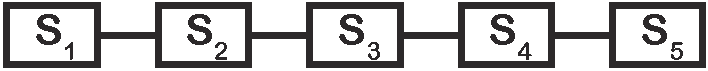
\includegraphics[width=0.6\linewidth]{pic/exam-topo5.pdf}
    \caption{Example topology.
    }
    \label{fig:exam-topo5}
    \vspace{-0.1in}
\end{figure}

\begin{figure}[t]
    \centering
    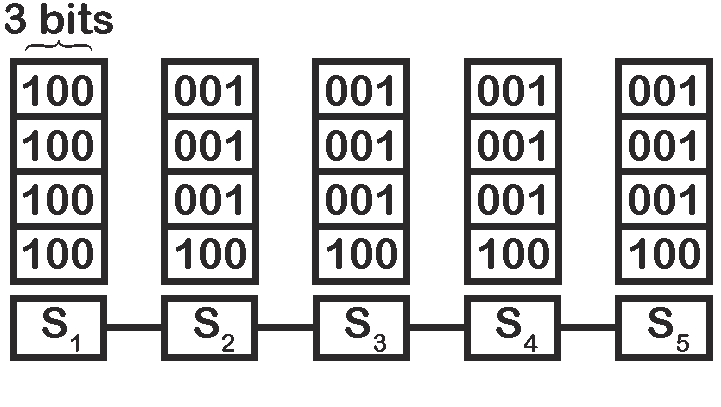
\includegraphics[width=0.6\linewidth]{pic/exam-fixed-width.pdf}
    \caption{Example of the counter arrays for the traditional large fixed-width counter solution.
    }
    \label{fig:exam-fixed-width}
    \vspace{-0.1in}
\end{figure}

The fixed-width approach always assumes the worst case, \ie, each switch will allocate 4 counters for elephant flows, no matter in average or dominant case.
As a result, it takes 60 bits in total, since a 4-byte elephant flow takes 3 bits for counting, as shown in Fig.~\ref{fig:exam-fixed-width}.
BRICK can largely save the memory in the average case, because it can flexibly extend the 1-bit bucket.
As shown in Fig.~\ref{fig:exam-brick-avg}, it consumes 30 bits in total to handle all possible average cases.
However, in dominant cases, BRICK also has to allocate 12 bits for each switch, since it cannot predict which switch will be the hot spot, as shown in Fig.~\ref{fig:exam-brick-dmn}.
In other words, in this simple example, BRICK will consume the same memory with the fixed-width approach, if it wants to avoid exceeding the switch memory in any possible case.

We note that in practice, we have bare knowledge of the flow numbers and sizes.
This fact will benefit the actual performance of BRICK, since it can adaptively extend the counter.
However, the above analysis also shows that BRICK may still fail the counting if too many elephant flows are counted in a single switch.

\begin{figure}[t]
    \centering
    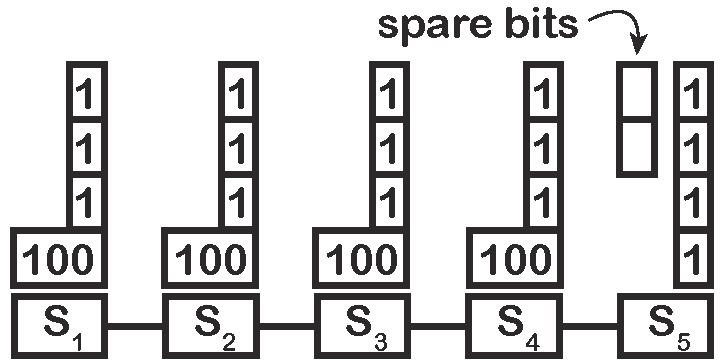
\includegraphics[width=0.6\linewidth]{pic/exam-brick-avg.pdf}
    \caption{Example of the average case of the counters for BRICK.
     }
    \label{fig:exam-brick-avg}
\end{figure}

\begin{figure}[t]
    \centering
    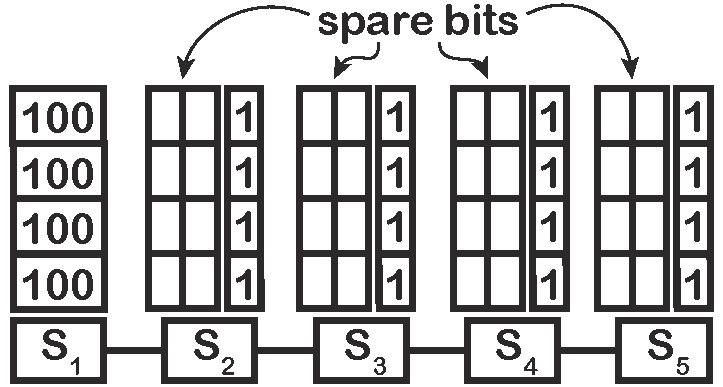
\includegraphics[width=0.6\linewidth]{pic/exam-brick-dmn.pdf}
    \caption{Example of the dominant case for BRICK.
     }
    \label{fig:exam-brick-dmn}
\end{figure}

\subsection{Basic Idea of DIAL}\label{sec:to-idea}
We propose DIAL based on a simple observation:
recall the worst case of BRICK shown in Fig.~\ref{fig:exam-brick-dmn}, when the gathered elephant flows impact the memory in a single switch, much memory remains unused in others.
Therefore, our basic idea is to exploit the spared memory in other switches as a supplement to the local memory, so that the elephant flows can be jointly counted by multiple switches instead of a single one.
Still considering the aforementioned example, we use $f_1$--$f_{20}$ to denote the 20 flows in the network, where $f_1$--$f_4$ are the 4-byte elephant flows.
DIAL allocates a set of 1-bit counters for each switch, and when a specific counter is exceeded, DIAL will use a spared counter in other switches to continue counting the flow.
Fig.~\ref{fig:exam-dial-dmn8} depicts one of the dominant cases, where all elephant flows are originally counted in the first switch.
It can be seen that 8 bits for each switch are sufficient.
For this worst case, the total memory cost is 40 bits, which is lower than that of the fixed-width approach and BRICK.
Plus, DIAL in the average case has a similar cost.

Though the above analysis shows the potential benefit of DIAL, we note that DIAL could bring much overhead if being simply applied.
The reason is that to implement the supplementary counters along a routing path, the original counting rule must be duplicated.
To be specific, DIAL has to duplicate all the counting rules to all the switches, in case any of them becomes an elephant flow.
This duplication makes DIAL impracticable for two reasons.
First, the number of counting rules increases with the number of switches, which largely consumes the flow entries in the flow table.
For example in Fig.~\ref{fig:exam-dial-dmn8}, the 20 flows will consume 100 flow entries.
Second, the counter memory is occupied right after the counting rules are installed.
That is, the counting memory cost will also increase with the number of switches.
For example in Fig.~\ref{fig:exam-dial-dmn8}, even assuming we have the pre-knowledge that there are only 4 elephant flows and that 8 bits for each switch are sufficient, DIAL still has to allocate 100 bits, since we don't know which four could grow to be elephant.

\begin{figure}[t]
    \centering
    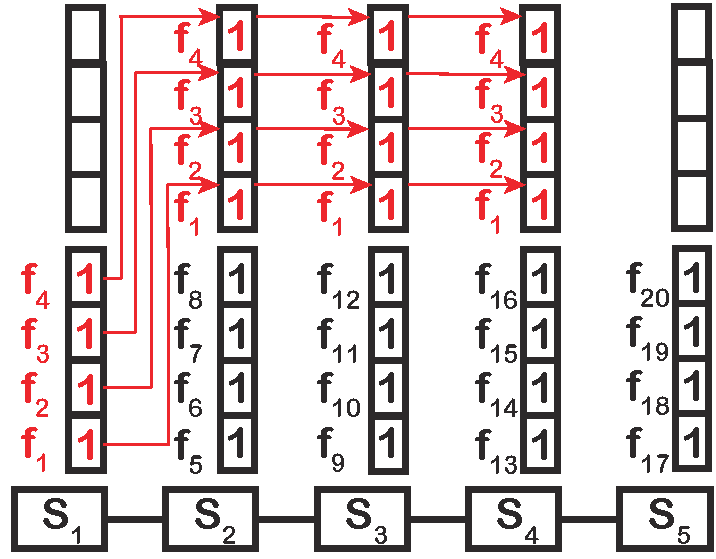
\includegraphics[width=0.6\linewidth]{pic/exam-dial-dmn8.pdf}
    \caption{Example of the dominant case for DIAL.}
    \label{fig:exam-dial-dmn8}
    \vspace{-0.2in}
\end{figure}

\section{Adaptive Counting Rule Duplication}\label{sec:dup}
\subsection{Counting Rule Duplication Problem}\label{sec:dup-prob}
Recall the 80/20 rule indicating only a small portion of flows are elephant flows, duplicating all the counting rules will waste lots of flow entries.
A straightforward method is to adaptively duplicate the counting rules for those flows that cannot be counted in their original switches.
However, considering there could be multiple flows requiring extra counting rules simultaneously, the arbitrary duplication may produce the hot spot where the switch runs out of its flow table entries and/or counting memory.
That is, we must carefully decide where to duplicate the rule for each flow, namely counting rule duplication problem (CRDP).

We formalize CRDP as follows.
Assume there are $N$ switches in total, and $M$ flows requiring extra counting rules.
If we duplicate a counting rule for flow $M_i$ to switch $N_j$, it will consume $a_{ij}$ counting memory along with $b_{ij}$ flow table entries.
If $M_i$ cannot be assigned to $N_j$, \ie, $N_j$ is not in the routing path of $M_i$, $a_{ij}$ and $b_{ij}$ will be infinite.
Note that $b_{ij}$ does not always equal to 1, because the counting rule may have to be further divided to fit into the original flow table.
In sum, CRDP can be formalized by the following model:
\begin{eqnarray}
\text{minimize}  & \displaystyle\sum\limits^{M}_{i=1} a_{ij}x_{ij}\sum\limits^{M}_{i=1} b_{ij}x_{ij} & j=1,...,N\\
\text{subject to}& \displaystyle\sum\limits^{M}_{i=1} a_{ij}x_{ij}\leq A_j,  & j=1,...,N \\
                 & \displaystyle\sum\limits^{M}_{i=1} b_{ij}x_{ij}\leq B_j,  & j=1,...,N \\
                 & \displaystyle\sum\limits^{N}_{j=1}x_{ij}=1,  & i=1,...,M
\end{eqnarray}

Eq. (1) is to minimize the cost of counting memory and flow entries.\footnote{The weights of the two parts are unknown, so we multiply (not add) them.}
Eq. (2) and Eq. (3) constrain the counting memory and number of flow entries.
Eq. (4) defines a 0-1 variable to represent that each rule can only be duplicated to one switch.
Actually, $a_{ij}$ is a constant value for all assignment ($M_i$ to $N_j$), since DIAL allocates same-size counters for each flow.
As a result, we could rewrite the objective to minimize the second factor, \ie, the number of flow entries.
In this way, CRDP captures the well-known Multi-Resource Generalized Assignment Problem (MRGAP), which has been proved to be NP-hard~\cite{doi:10.1287/mnsc.37.6.695}.

We note that $M$ could be relatively small in practice due to the limited number of elephant flows.
However, the first-time ``duplication'', \ie, the initial counting rule placement, involves all flows in the network, incurring a large overhead of computing optimal solution.
As a result, we still need to seek near-optimal solution for CRDP.

\subsection{Heuristics of Near-Optimal Duplication}\label{sec:dup-alg}
Due to the NP-hardness of CRDP, we propose some simple heuristics to approximately approach the optimal duplication solution under the acceptable time consumption.
Specifically, we consider the following requirements of duplication placement:
(1) the consumption of the two resources (counting memory and \#flow entries) should not go beyond their capacities, and
(2) the consumption of the two resources should be balanced for all switches.

The heuristics is to greedily find the lightest-loaded switch to duplicate the counting rule for each flow that exceeds its original counter, namely Lightest-Loaded-First duplication (LLF).
We note that, for a certain flow, the number of candidate switches for duplication is actually the number of hops of this flow.
That is, flows with longer path have more options to place the duplicated rules.
As a result, for a bunch of flows to be duplicated, LLF will first decide the duplication place for the flows with shorter path.

Algorithm~\ref{alg:place} depicts the whole process of finding a near-optimal duplication solution.
To be specific, \texttt{multi\_place} works out the priority of all the duplicating flows by their routing paths' length, and \texttt{place} finds the lightest-loaded switch from the candidates for each duplicating flows sequentially.

For example in Fig.~\ref{fig:exam-dial-place}, each switch counts four flows in the beginning.
Suppose that the routing paths of $f_1$ and $f_2$ are $S_1 \rightarrow S_2$ and $S_1 \rightarrow S_2\rightarrow S_3$, respectively.
If afterwards both $f_1$ and $f_2$ in $S_1$ need to duplicate their counting rules, \texttt{multi\_place} will first arrange to \texttt{place}($f_1$) that has a shorter routing path.
For $f_1$, only $S_2$ is available, so it duplicates the rule to and creates a 1-bit counter in $S_2$.
Next, \texttt{place}($f_2$) is called, and here $S_3$ is lighter loaded than $S_2$, so the duplicated rule will be placed in $S_3$.

\begin{figure}
    \centering
    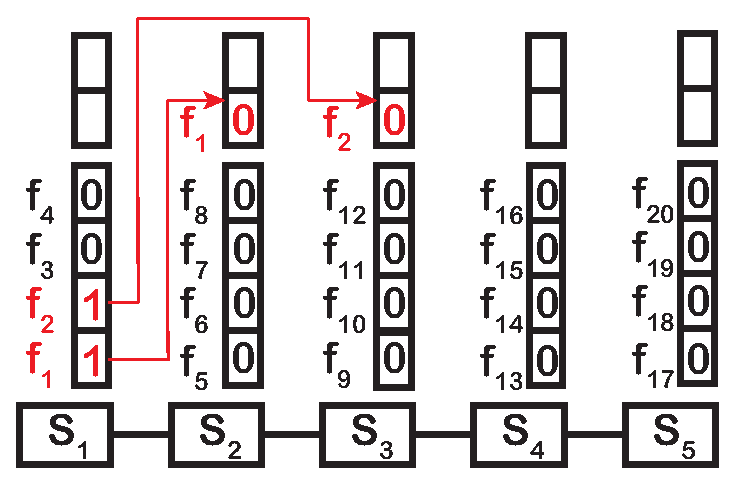
\includegraphics[width=0.6\linewidth]{pic/exam-dial-place}
    \caption{Example of the duplication for DIAL.}
    \label{fig:exam-dial-place}
\end{figure}

\begin{algorithm}[t]\small
\caption{Lightest-loaded-first duplication}
\label{alg:place}
\KwIn{\KwOut{the set of flows to be duplicated: $fs$}}
\BlankLine
\texttt{multi\_place}($fs$)
\Begin{
     sort $fs$ in ascending order of the number of available switches along the routing path of each flow\;
    \ForEach{$f\in fs$}{\texttt{place}($f$)\;}
}
\BlankLine
\texttt{place}($f$)
\Begin{
    $ss \leftarrow$ \{$s$ $|$ $s$ is along the routing path of $f$ and there is no rule of counting $f$ in $s$\}\;
    sort $ss$ in ascending order of the load of each switch\;
    $lis \leftarrow$ the lightest-loaded switch of $ss$\;
    install the rule of counting $f$ in $lis$\;
    create the counter of $f$ in $lis$\;
}
\end{algorithm}

\textbf{Pre-duplication.}
Ideally, the duplication happens only when the original counter exceeds.
However, this process has to wait for the controller to issue the new counting rule, which will incur large latency through each duplication.
We employ a pre-duplication process into DIAL to mitigate the latency problem.
Specifically, after initially placing the counting rules, we directly duplicate them by re-running \texttt{multi\_place} of LLF in Algorithm~\ref{alg:place}.
That is, all the counting rules are at least duplicated once.
When a flow exceeds its first counter, a third one will be allocated immediately.
As a result, the controller has plenty of time to issue the new counting rule, as long as the second counter is not full.
In this way, elephant flows are properly counted without employing extra latency.

Fig.~\ref{fig:exam-dial-predup} depicts a possible result after the pre-duplication, in which the assumptions are the same as those in Fig.~\ref{fig:exam-dial-dmn8}.
After duplicating all the counting rules once, each switch counts eight flows now.
It can be seen that $f_1$ has two counters in $S_1$ and $S_2$ at the start, and the one in $S_1$ is counting the first byte of $f_1$.
When $f_1$ exceeds its counter in $S_1$, \texttt{overflow\_report} in Algorithm~\ref{alg:handle} will \texttt{place}($f_1$) in another switch, $S_3$. Meanwhile, the elephant flow $f_1$ can be properly and continuously counted in $S_2$.

\begin{figure}
    \centering
    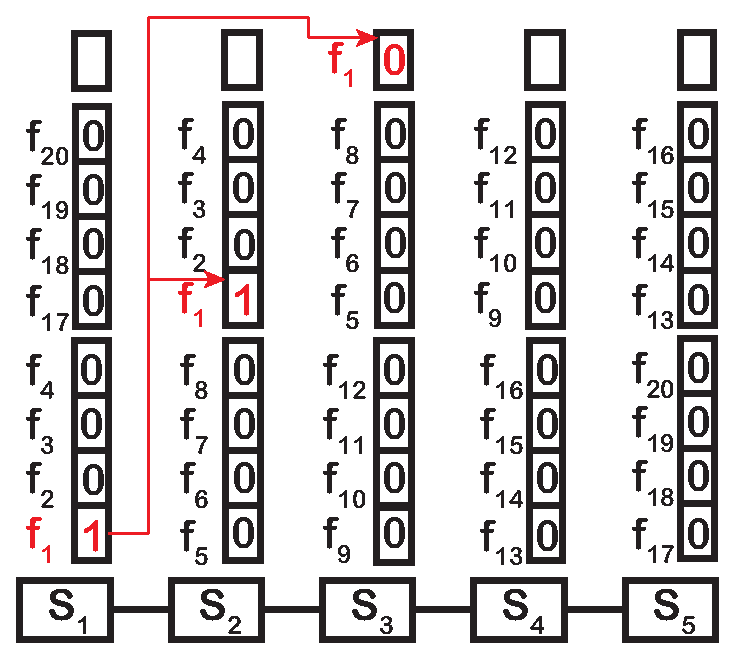
\includegraphics[width=0.6\linewidth]{pic/exam-dial-predup}
    \caption{Example of the pre-duplication for DIAL.}
    \label{fig:exam-dial-predup}
    \vspace{-0.1in}

\end{figure}

\section{Enforce DIAL into SDN}\label{sec:imp}
In this section, we highlight some key designs of enforcing DIAL into real SDN environment.

\textbf{Tag packets.}
To avoid redundant counting in the switches along the routing path of a specific flow, the first switch that counts the flow should tag the packet as ``counted''.
In OpenFlow, we can tag packets using an unused field of packet, \eg, VXLAN.
Such field will be initialized with 0, denoting ``uncounted''.
All the counting rules should only match the uncounted packets.
In real time matching, if a packet is matched with a counting rule, the rule should modify the field to be 1, \ie, the packet has been counted.

\textbf{Update results.}
In the measurement system, the controller will collect the counters of all switches periodically.
To be specific, at the end of each measurement period, switches will report their counter values to the controller by calling \texttt{upload} in Algorithm~\ref{alg:handle}.
This can be implemented by Statistics messages in OpenFlow for querying the counters.

\textbf{Handle exceptions.}
In real-time counting, if a counter exceeds, \texttt{overflow\_report} in Algorithm~\ref{alg:handle} will be triggered to set the switch to be ``FULL''.
If it doesn't exceed, this packet of the flow will remain ``uncounted'' and pass the switches which contain no rule or have been ``FULL'' for the flow.
If all switches of a flow are full or have installed the counting rule, then \texttt{upload} will be triggered to upload the statistics of the flow in all switches to the controller counters and then clear the counter values in the switches to continue counting.
During the counting process of DIAL, when a counter exceeds, the duplication happens as \texttt{overflow\_report} is triggered.
In this procedure, an integer is used to help index the switch which incurs the overflowing.
Then the flow will set the switch ``FULL'' and call \texttt{place} to find another switch to count it on.

In OpenFlow, \texttt{overflow\_report} and \texttt{upload} launched by switch-end can be implemented with Flow-monitor, Experimenter, and Packet\_in messages in special cases.

\begin{algorithm}[t]\small
\caption{Exception handling}
\label{alg:handle}
\KwIn{\KwOut{the flow to be handled: $f$}}
\BlankLine
\texttt{upload}($f$)
\Begin{
	\ForEach {$s$ along the routing path of $f$} {
		\If {the rule of counting $f$ has been installed in $s$}
		{
            upload the counter value of $f$ in $s$ to the controller and update the corresponding controller counter\;
            reset the counter value of $f$ in $s$ to zero\;
            set the state of $s$ along the routing path of $f$ to ``COUNTING''\;
		}
	}
}
\BlankLine
\texttt{overflow\_report}($f$, $i$)
\Begin{
    \If {a packet leads to an overflow} {
        set the state of the $i$-th switch along the routing path of $f$ to ``FULL''\;
		\texttt{place}($f$)\;
    }
}
\end{algorithm}
\vspace{-2ex}

\section{Evaluation}\label{sec:eval}
\subsection{Settings}
In this section, we evaluate the performance of DIAL.
Since DIAL is complementary to the optimization in a single switch, we involve the fixed-width and variable-width approaches in our evaluation.
The placement of the counting rules is critical for the above two approaches.
We specifically simulate three cases:
(1) randomly select the original counting switch for each flow,
(2) choose the most empty switch to count the flow (\ie, LLF), and
(3) apply DIAL with adaptive rule duplication.

We use three public real-world Internet traffic traces collected in 2016 from CAIDA~\cite{CAIDA} in our evaluation.
Each trace has about 1M flows and the largest flow needs a 28/29-bit width counter.
As shown in Table~\ref{tab:result}, each trace has a theoretical optimum (T. O.) memory cost which is calculated by the sum of every theoretical minimal counter width of each flow.

We employ two real-world network topologies from the Internet Topology Zoo~\cite{6027859}, \ie, CERNET (36 switches) and ChinaNet (38 switches).
We further involve a simulated topology based on fat-tree ($k=4$).
Given the topologies, we simulate the hosts by evenly partitioning all IPv4 addresses\footnote{class A, B and C are included but class D and E are excluded~\cite{Classful_network}} and distributing them to the edge switches.
The routing path for each packet class (source and destination IP pair) from the traces is then generated by the shortest-path algorithm.

We consider the following two metrics:
(1) the total memory cost, and
(2) the memory efficiency.
Here the memory efficiency is defined as the ratio of the theoretical optimum to the actual memory cost in total, since all the involved approaches are inevitable to waste some of the memory.
We assume the ideal cases for fixed- and variable-width approaches when calculating the total memory cost:
for fixed-width approach, we do not set the counter width beforehand, but use the actual consumed memory to calculate the total cost, which avoids the memory exceeding or unnecessary memory waste;
for variable-width approach, we assume it has a set of 1-bit buckets without extra overhead (\eg, pointer to link multiple buckets), which could maximize the memory efficiency in a single switch.
For DIAL, we assume a threshold of 13-bit width, which means the global counting mechanism will be triggered if the local counter exceeds 13-bit memory.
This threshold can be adaptively adjusted for different situations.

\subsection{Results}
Fig.~\ref{fig:memory-cost} depicts the total memory cost of all six approaches.
It can be seen that DIAL can largely decrease the memory cost, no matter combined with fixed- or variable-width approach.
Specifically, if we apply DIAL to the fixed-width approach, the memory cost will be reduced by 82\%--93\% and 57\%--88\%, compared to random and LLF placement, respectively.
The variable-width approach has drawn a similar trend by applying DIAL:
the memory cost will be reduced by 58\%--78\% and 7\%--54\%, respectively.

Additionally, the memory efficiency of these six approaches is shown in Fig.~\ref{fig:memory-efficiency}.
It can be observed that DIAL can significantly increase the memory efficiency for both fixed- and variable-width counter approaches.
To be specific, when DIAL is applied to the fixed-width approach, the results of memory efficiency reveal that it will bring about 459\%--1320\% increases if compared to random placement, and 133\%--688\% rises if compared to LLF placement.
The effect of using DIAL is also satisfying with the variable-width counter approach:
the memory efficiency will be raised by 139\%--338\% and 55\%--207\%, compared to the two placements respectively.

\begin{figure}[t]
\centering
\vspace{-0.2in}
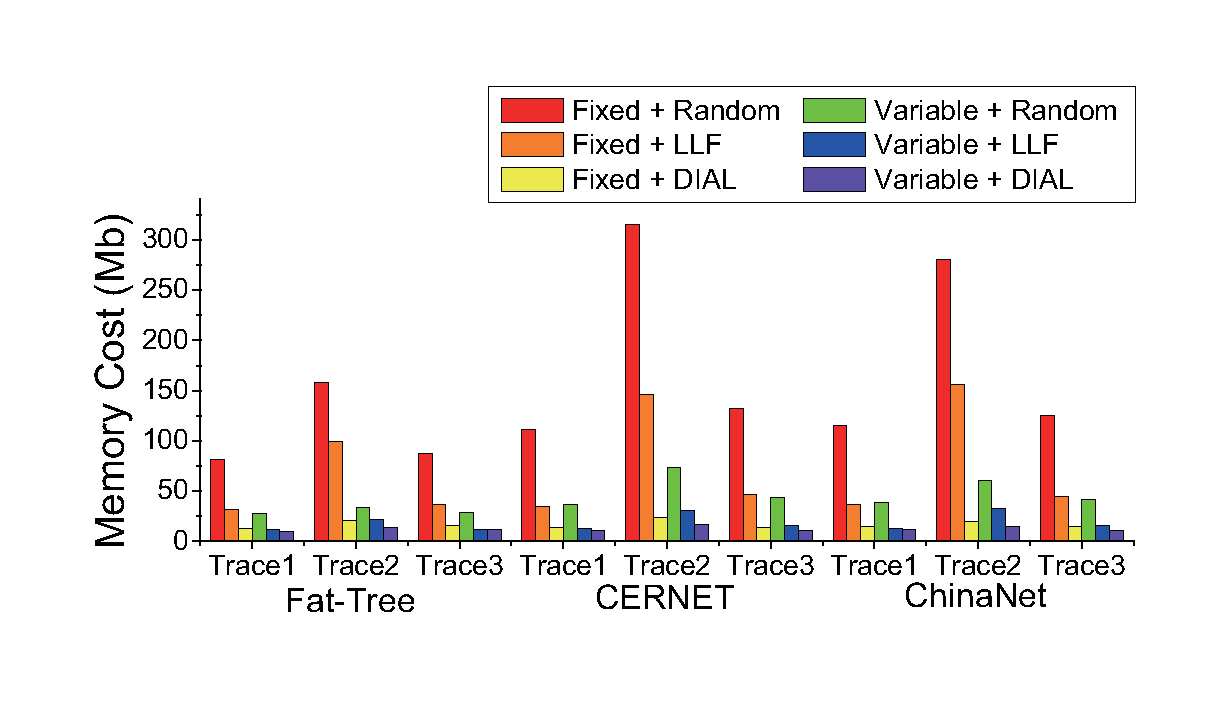
\includegraphics[width=0.5\textwidth]{data/cost}
\vspace{-0.4in}
\caption{Memory cost}
\label{fig:memory-cost}
\vspace{-0.2in}
\end{figure}

\begin{figure}[t]
\centering
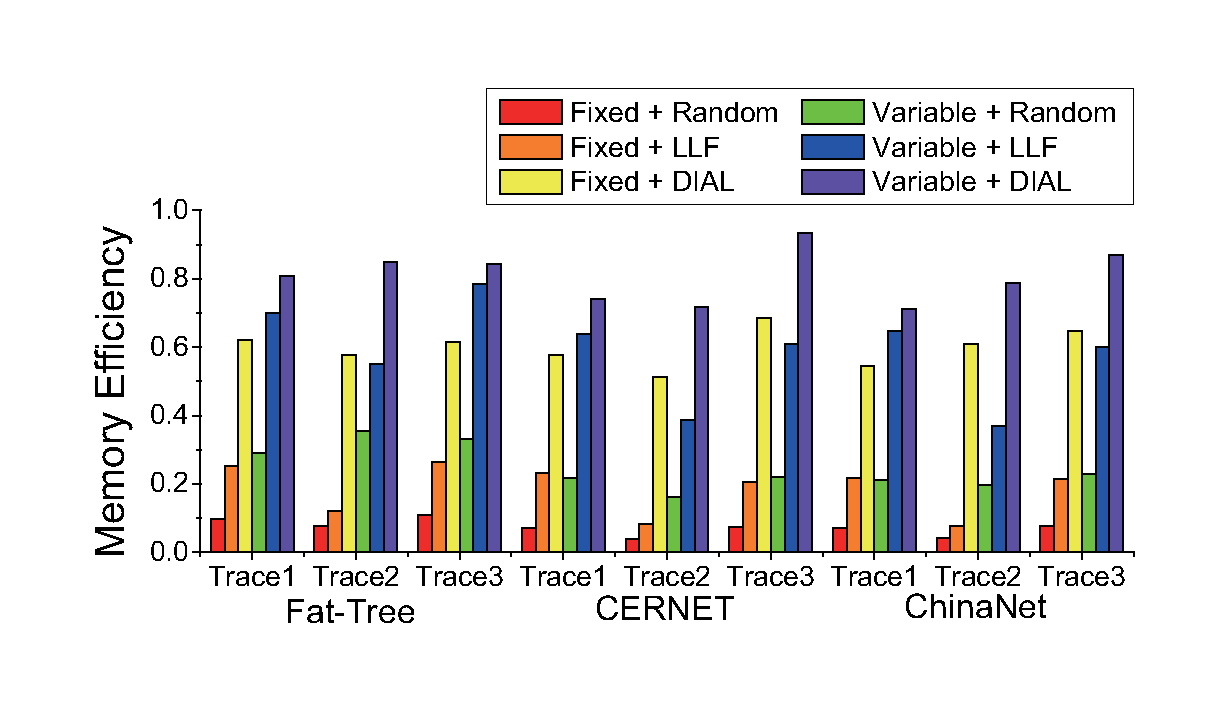
\includegraphics[width=0.5\textwidth]{data/efficiency}
\vspace{-0.4in}
\caption{Memory efficiency}
\label{fig:memory-efficiency}
\vspace{-0.2in}
\end{figure}

We further measure the overhead of extra Packet\_in messages when handling exceeding exceptions, as is denoted in the ``Costs'' field in Table~\ref{tab:result}.
We find that the ``Costs'' count is at the same order of magnitude with the flow count.
We know that in periodic network measurement in SDN, one flow has to lead the switch to communicate with the controller at least once when submitting the result at the end of the measurement period.
In DIAL, the extra message cost is introduced, which leads to an increase in the number of the same messages \eg, Packet\_in costs in OpenFlow, but that is still at the same order of magnitude, so we consider that it is endurable with high bandwidth SDN link. For example, the system in~\cite{Liu2017} has the 1Gbps SDN link.

\begin{table}[t]\small
 \caption{Some results of DIAL}
  \label{tab:result}
  \centering
  \begin{tabular}{ccccc}
    \toprule
    Topology & Trace  & \#Flow & T. O.  & Costs\\
    \midrule
    Fat-Tree & Trace1 & 0.9M   & 8.08Mb & 2.0M \\
    Fat-Tree & Trace2 & 1.5M  & 12.0Mb & 3.5M \\
    Fat-Tree & Trace3 & 1.0M  & 9.61Mb & 2.7M \\
    CERNET   & Trace1 & 0.9M   & 8.08Mb & 1.9M \\
    CERNET   & Trace2 & 1.5M  & 12.0Mb & 3.4M \\
    CERNET   & Trace3 & 1.0M  & 9.61Mb & 2.2M \\
    ChinaNet & Trace1 & 0.9M   & 8.08Mb & 1.9M \\
    ChinaNet & Trace2 & 1.5M  & 12.0Mb & 3.2M \\
    ChinaNet & Trace3 & 1.0M  & 9.61Mb & 2.3M \\
    \bottomrule
  \end{tabular}
  \vspace{-2ex}
\end{table}

\section{Related Work}\label{sec:rel}
\textbf{Fixed-width counter.}
In flow statistics field, many approaches have been proposed to save the on-chip memory.
DISCO~\cite{Hu2010} elaborately designs the counter update rule so that the increment of the updated counter is less than the actual packet length.
ANLS~\cite{Hu2012} uses a sampling technique and dynamically sets a smaller sampling rate when the counter value is large, to reduce the memory usage.
These approaches can save memory cost, but they still apply fixed-width counters, leading to low memory efficiency.

\textbf{Variable-width counter.}
To save the memory wasted by fixed counter width, variable-width counter architecture has been proposed.
BRICK~\cite{Hua2008} is the state-of-the-art variable-width counter approach.
BRICK splits a counter into several sub-counters, and will allocate an extra sub-counter to a flow only when it exceeds the original memory size.
However, in the cases of multiple per-flow tasks, BRICK may fail when handling the hot spots of elephant flows.

DIAL is complementary to these approaches.
As a result, a smaller counter/bucket can be set with much lower risk of memory exceeding, so as to further reduce the overall cost.
For example, OpenCounter~\cite{Callegari2015} counts unknown flows in SDN, maintaining a counter named LLCRS in the controller for each switch, and aggregates them when queried. 
The design philosophy of OpenCounter is similar to DIAL. 
Both of them are distributed counting architecture based on SDN. 
However, OpenCounter focus on unknown flow counting in controller, with specific data structure LLCRS, whereas DIAL can count any flows in switch, with diverse data structure options, depending on the specific usage, which is a more general counting architecture framework.
\section{Conclusion}\label{sec:con}
In this paper, we explored the memory waste problem of per-flow counting.
Specifically, we propose a distributed counting approach on SDN, \ie, DIAL.
In contrast to only focusing on reducing the local switch memory, DIAL leverages the spared memory along the routing path to make a global optimization.
In this work, we formulate the problem of finding the optimal placement for the extra counting rules, and propose simple heuristics to fast generate a near-optimal solution.
The evaluation based on real and synthetic traces and topologies has demonstrated that DIAL is effective, efficient and scalable with various local optimization approaches.

\section*{Acknowledgment}
This work is supported by the National Key Research and Development Program of China (2017YFB0801703), NSFC (61702407, 61672425), and Fundamental Research Funds for the Central Universities.
% The authors would like to thank...

\bibliographystyle{IEEEtran}
\bibliography{network}

\end{document}
